\newpage
\section{Resultados}

\subsection{Rede $L$}

Foram calculados os parâmetros dos componentes da rede L, chegando-se no circuito mostrado na figura \ref{f_sch_rede_L}.

\begin{figure}[H]
    \centering
    \caption{Circuito da rede L.}
    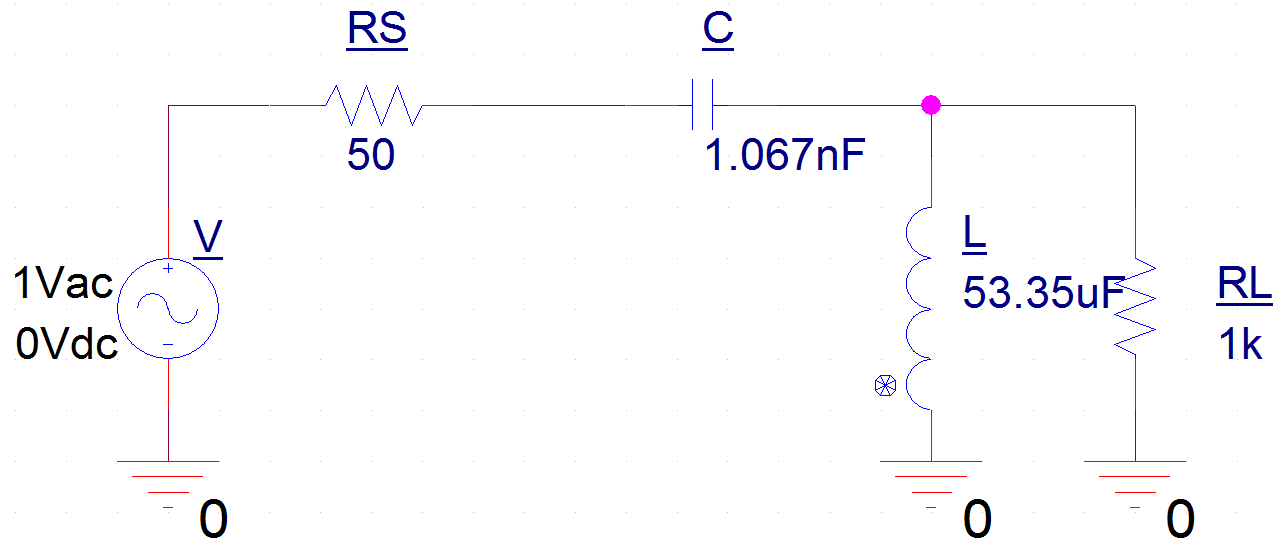
\includegraphics[scale=0.4]{Imagens/sch_rede_L.png}
    \label{f_sch_rede_L}
\end{figure}

O circuito foi então simulado no modo AC-Sweep, onde foi obtido o gráfico da figura \ref{f_rede_L_graph}.

\begin{figure}[H]
    \centering
    \caption{Resposta em frequência da rede L.}
    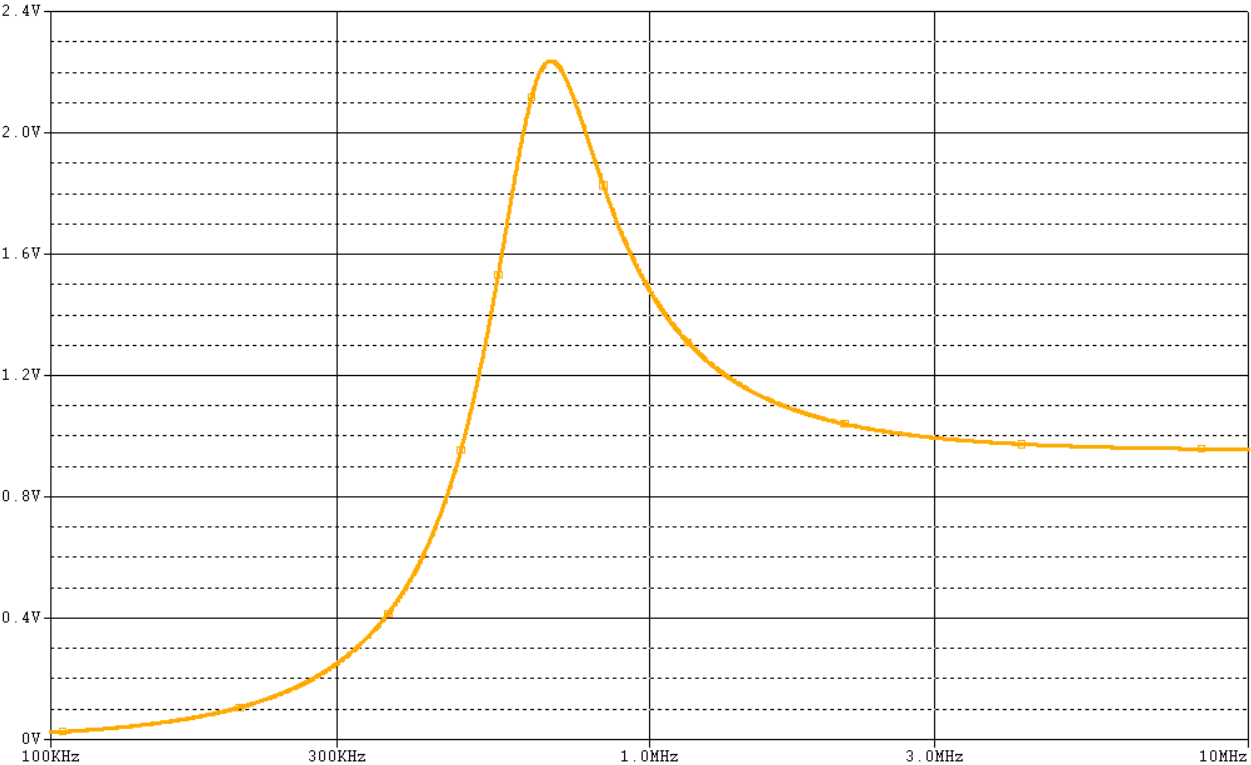
\includegraphics[scale=0.4]{Imagens/rede_L_graph.png}
    \label{f_rede_L_graph}
\end{figure}

Foram obtidos os seguintes dados para a rede L:\\
 - $F_c$ = 683,912 kHz. \\
 - $BW3db$ = 30kHz. \\ 
 - $BW potência$ = 17,25 kHz. \\ 
 - Fator $Q$ = 4.6. \\
 
 \subsection{Rede $L_{wideband}$}
 
 Foram calculados os parâmetros dos componentes da rede $L_{wideband}$, chegando-se no circuito mostrado na figura \ref{f_sch_rede_L_wideband}.
 
 \begin{figure}[H]
     \centering
     \caption{Circuito da rede $L_{wideband}$.}
     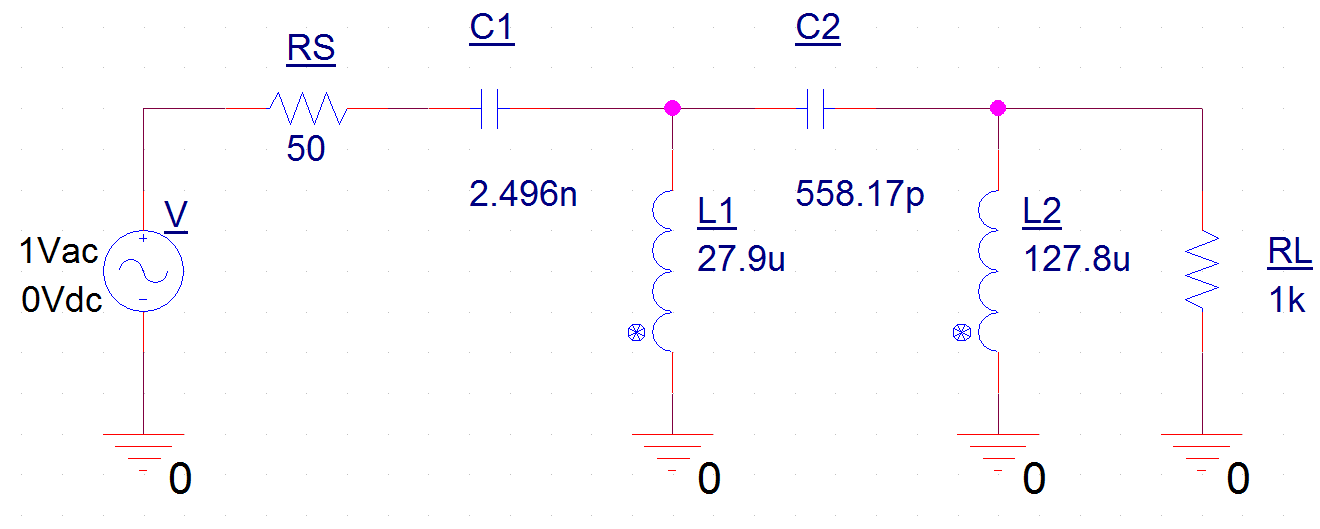
\includegraphics[scale=0.4]{Imagens/sch_rede_L_wideband.png}
     \label{f_sch_rede_L_wideband}
    \end{figure}
    
    O circuito foi então simulado no modo AC-Sweep, onde foi obtido o gráfico da figura \ref{f_rede_L_wideband_graph}.
    
    \begin{figure}[H]
        \centering
        \caption{Resposta em frequência da rede $L_{wideband}$L.}
        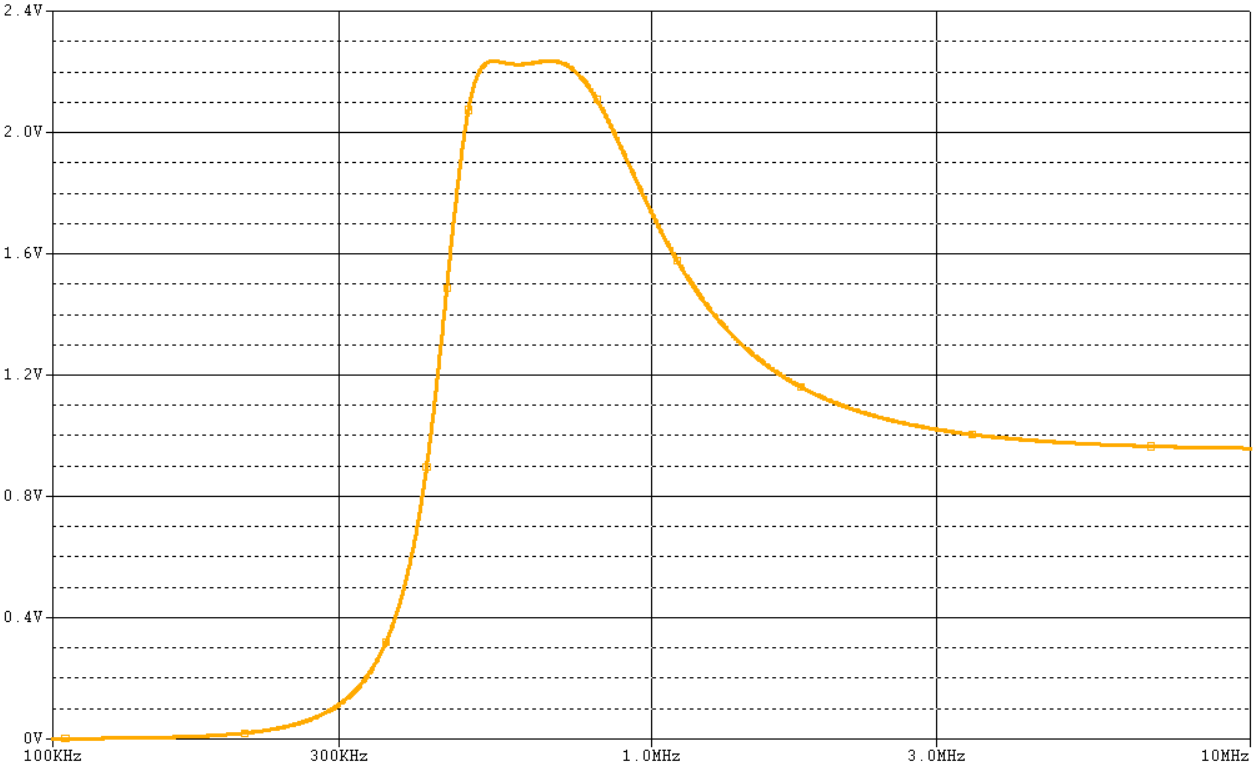
\includegraphics[scale=0.4]{Imagens/rede_L_wideband_graph.png}
        \label{f_rede_L_wideband_graph}
    \end{figure}
    
    Foram obtidos os seguintes dados para a rede $L_{wideband}$:\\
    - $F_c$ = 684,312 kHz. \\
    - $BW3db$ = 352,981kHz. \\
    - $BW potência$ = 197,563 kHz. \\
    - Fator $Q$ = 2.8. \\
 
 
 \subsection{Rede $T$}
 
 Foram calculados os parâmetros dos componentes da rede $T$, chegando-se no circuito mostrado na figura \ref{f_sch_rede_T}.
 
 \begin{figure}[H]
     \centering
     \caption{Circuito da rede T.}
     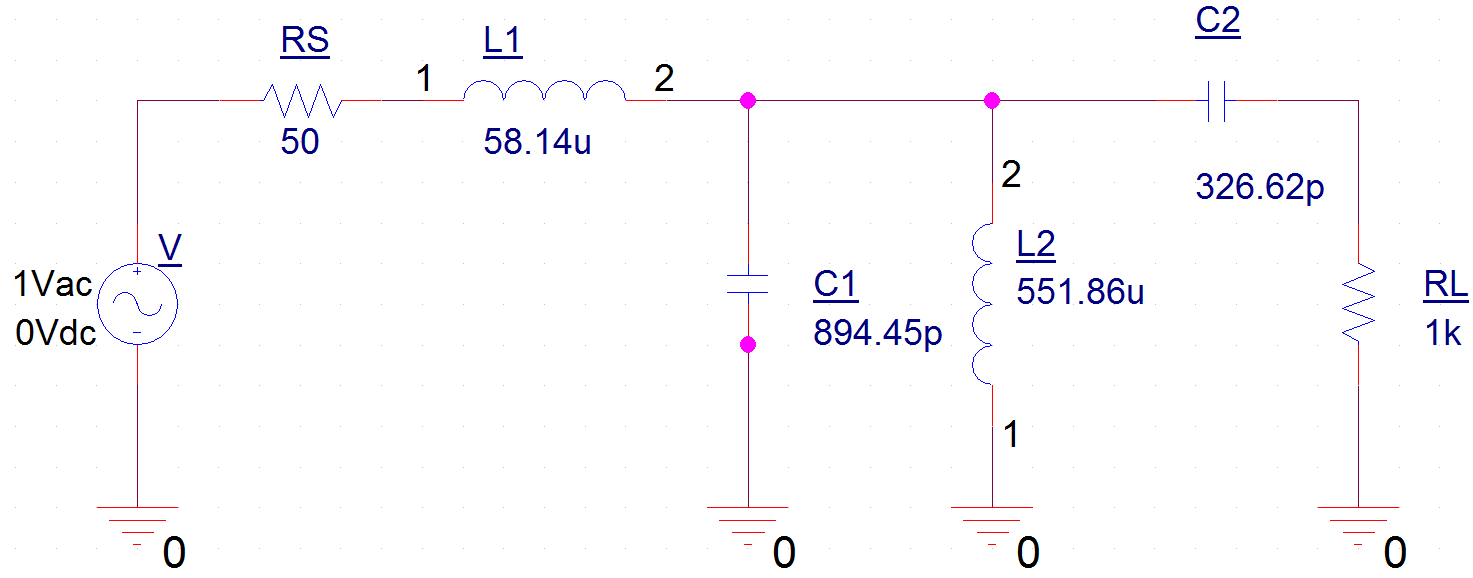
\includegraphics[scale=0.4]{Imagens/sch_rede_T.png}
     \label{f_sch_rede_T}
    \end{figure}
    
    O circuito foi então simulado no modo AC-Sweep, onde foi obtido o gráfico da figura \ref{f_rede_T_graph}.
    
    \begin{figure}[H]
        \centering
        \caption{Resposta em frequência da rede T.}
        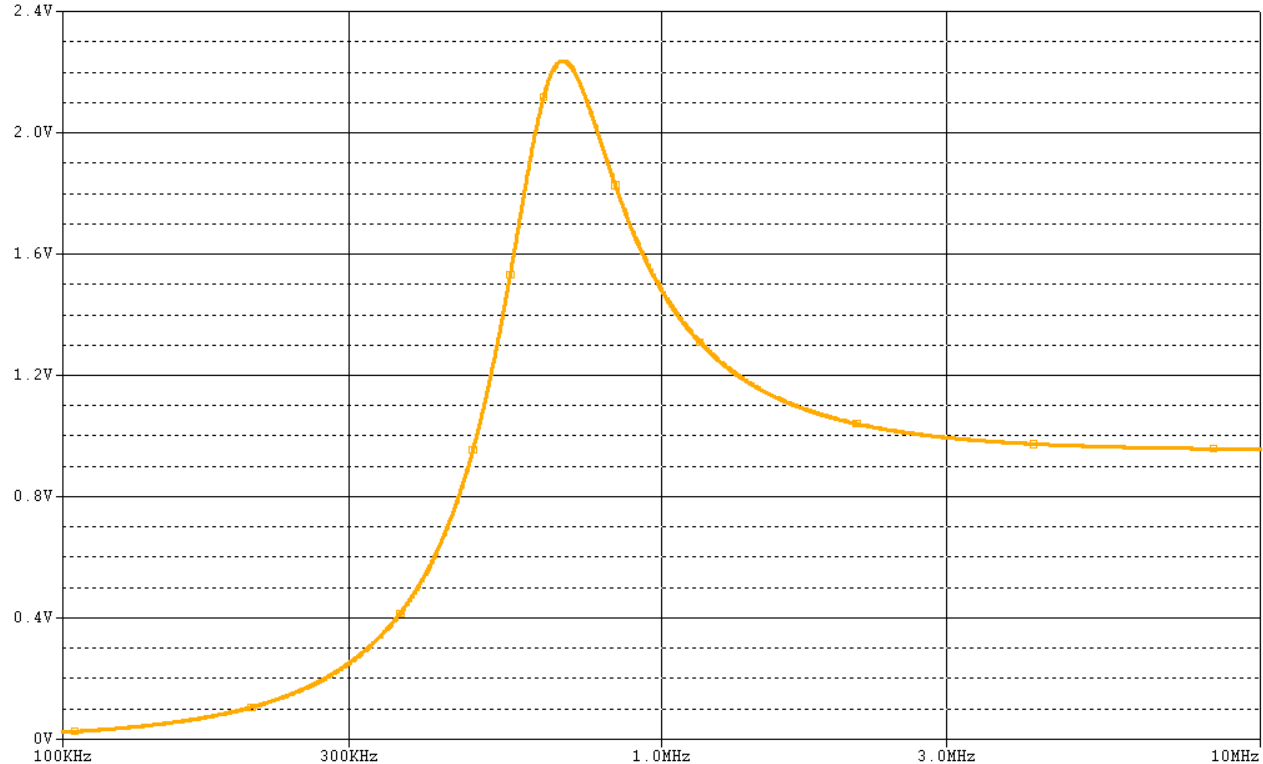
\includegraphics[scale=0.4]{Imagens/rede_T_graph.png}
        \label{f_rede_T_graph}
    \end{figure}
    
    Foram obtidos os seguintes dados para a rede T:\\
    - $F_c$ = 687,21 kHz. \\
    - $BW3db$ = 160,16 kHz. \\
    - $BW potência$ = 100,278 kHz. \\
    - Fator $Q$ = 6.8. \\